
\documentclass[a4paper,11pt]{article}


%%% fontenc
%\usepackage{fontspec,xunicode,xltxtra}
%\setmainfont{Times New Roman}
%\setsansfont{Source Sans Pro}
%\setmonofont{Source Sans Pro}

%%% xeCJK
\usepackage{xeCJK}
\setCJKmainfont[BoldFont=Adobe Heiti Std]{Adobe Song Std}
\setCJKsansfont[BoldFont=Adobe Heiti Std]{Adobe Song Std}
\setCJKmonofont[BoldFont=Adobe Heiti Std]{Adobe Song Std}
\XeTeXlinebreaklocale "zh"
\XeTeXlinebreakskip=0pt plus 1pt minus 0.1pt

\usepackage{xcolor}
\usepackage{graphicx}

%%% get total page number
\usepackage{lastpage}

%%% customized definition
\makeatletter
\def\sybtitle#1{\def\@sybtitle{#1}}
\def\sybauthor#1{\def\@sybauthor{#1}}
\def\sybdate#1{\def\@sybdate{#1}}
\sybtitle{}
\sybauthor{}
\sybdate{}
\def\sybmaketitle{
  \begin{center}
  \vspace*{.8in}
  {\huge\bfseries\@sybtitle}
  \par
  \vspace{.8in}
  {\Large\@sybauthor}
  \par
  \vspace{.2in}
  \@sybdate
  \vspace{.5in}
  \end{center}
}
\makeatother
\setlength{\parindent}{0pt}
\renewcommand{\today}{\number\month 月 \number\day 日, ~\number\year 年}
\def\lt{\textless}
\def\gt{\textgreater}
\renewcommand\contentsname{\bfseries 目~~录}
\newcommand\bs{\texttt{\symbol{'134}}} % input backslash sign
%\newcommand\bs{\string\} % same as above definition
\long\def\cmd#1{\par\vspace{.5em}\hspace*{2em}#1\vspace{.5em}\par}
\def\cstr#1{\texttt{\string#1}} % e.g. \cstr{\latex}
\long\def\runcode#1{\par\bigskip#1\bigskip\par}
% 我不想看到那么多的underful hbox,尤其是minted环境加上背景色之后
\hbadness=10000
% 适当放宽overful hbox的限制,运行2pt的溢出
\hfuzz=2pt
\parskip=3\lineskip


%%% change background color & add frame for enumerate enviroment
\usepackage{mdframed}
\newmdenv[backgroundcolor=blue!10,linewidth=0pt]{coloredframe}
\newenvironment{coloredenumerate}{
  \begin{coloredframe}
  \begin{enumerate}
}{
  \end{enumerate}
  \end{coloredframe}
}

%%% geometry
\usepackage[includehead,includefoot,hmargin=21mm,vmargin=10.5mm,
            headsep=12pt,headheight=25pt]{geometry}
%\usepackage[includehead,includefoot,hmargin=1.2in,vmargin=1in]{geometry}

%%% fancyhdr
\usepackage{fancyhdr}
\makeatletter
\fancypagestyle{main} {
  \fancyhf{} % clear header & footer
  \fancyhead[L]{\bfseries\@sybtitle}
  \fancyhead[R]{\thepage/\pageref*{LastPage}}
  \renewcommand{\headrulewidth}{0.4pt} % header line
  \renewcommand{\footrulewidth}{0pt} % footer line
}
\fancypagestyle{header} {
  \fancyhf{} % clear header & footer
  \fancyfoot[C]{\roman{page}}
  \renewcommand{\headrulewidth}{0pt} % header line
  \renewcommand{\footrulewidth}{0pt} % footer line
}
\makeatother

\usepackage{titlesec}
\titleformat{\part}{\centering\Large\bfseries}{第\,\thepart\,部分}{1em}{}
\titleformat{\section}{\large\bfseries}{\thesection}{1em}{}
\titleformat{\subsection}{\normalsize\bfseries}{\thesubsection}{1em}{}
%\titlespacing*{章节命令}{左边距}{上文距}{下文距}[右边距]
\titlespacing*{\section}{0pt}{2\baselineskip}{\parsep}


\usepackage{hyperref}

%%% perfect source code display
\usepackage{minted}
%\usemintedstyle{colorful}
\definecolor{srcbg}{rgb}{0.95,0.95,0.95}
\newminted{java}{linenos,tabsize=4,bgcolor=srcbg}
\newminted{xml}{linenos,tabsize=4,bgcolor=srcbg}
\newminted{cpp}{linenos,tabsize=4,bgcolor=srcbg}
\newminted{bash}{linenos,tabsize=4,bgcolor=srcbg}
\newminted{latex}{linenos,tabsize=4,bgcolor=srcbg}



\usepackage{xcolor}
\colorlet{HEADCOLOR}{red!50}
\colorlet{BRANCHCOLOR}{blue!50}
\colorlet{WORKCOLOR}{gray!50}
\colorlet{INDEXCOLOR}{cyan!50}
\colorlet{COMMITCOLOR}{green}

\usepackage{tikz}
\usetikzlibrary{shapes,arrows,positioning,calc,backgrounds,matrix,fit,decorations.pathreplacing}
\tikzset{
  basic-style/.style = {
    rectangle, rounded corners=2pt, draw, thick,
    fill=#1,
    minimum height=15pt,
    minimum width=1.5cm,
    inner sep=1pt
  },
  commit-style/.style = {
    basic-style=COMMITCOLOR
  },
  index-style/.style = {
    basic-style=INDEXCOLOR,
    minimum width=2.5cm
  },
  work-style/.style = {
    basic-style=WORKCOLOR,
    minimum width=2.5cm
  },
  branch-style/.style = {
    basic-style=BRANCHCOLOR
  },
  head-style/.style = {
    basic-style=HEADCOLOR
  },
  cmd-style/.style = {
    #1=5pt
  },
  cmd-style/.default = right,
  main-style/.style = {
    execute at end picture = {
      \begin{pgfonlayer}{background}
        \path[fill=gray!20,rounded corners]
          ([xshift=-0.2cm,yshift=-0.2cm]current bounding box.south west) rectangle
          ([xshift=0.2cm,yshift=0.2cm]current bounding box.north east);
          %(current bounding box.south west) rectangle
          %  (current bounding box.north east);
        \end{pgfonlayer}
    }
  },
  file-style/.style = {
    draw=red, fill=yellow!30, inner sep=2pt
  },
  dir-style/.style = {
    fill=green!50,inner sep=2pt
  },
  dir-bg-style/.style = {
    fill=cyan!30,rounded corners
  },
  every edge/.style = {draw, ->, >=latex', thick}
}

%%%%% new definitions %%%%%

\newlength\commitDistance
\setlength\commitDistance{0.5cm}
\newlength\indexWorkDistance
\setlength\indexWorkDistance{2\commitDistance}

\newcommand\displayName[1]{\ttfamily\bfseries #1}
\newcommand\commandName[1]{\ttfamily\bfseries\small #1}

\def\createNode style:#1 name:#2 display:#3 direct:#4 distance:#5 to:#6;{
  \node [#1, #4=#5 of #6] (#2) {#3}
        edge [#4] (#6);
}
\def\createCommit name:#1 display:#2 direct:#3 to:#4;{
  \node [commit-style, #3=\commitDistance of #4] (#1) {#2}
        edge [#3, COMMITCOLOR] (#4);
}
\def\createBranch name:#1 display:#2 direct:#3 to:#4;{
  \node [branch-style, #3=0.75\commitDistance of #4] (#1) {#2}
        edge [#3, BRANCHCOLOR] (#4);
}
\def\createHead direct:#1 to:#2;{
  \node [head-style, #1=0cm of #2] (head) {\displayName HEAD};
}
\def\createIndex to:#1;{
  \node [index-style, below=2\commitDistance of #1] (index) {\displayName Index};
}
\def\createWork to:#1;{
  \node [work-style, below=2\commitDistance of #1] (work) {\displayName Work DIR};
}

\newcommand\makeOutline{
  %\useasboundingbox (-0.1,-3.6) rectangle (10.7,2);
  \node[right] (dumy) at (0,0) {\dots};
  \createCommit name:a display:{\displayName A} direct:right to:dumy;
  \createCommit name:b display:{\displayName B} direct:right to:a;
  \createCommit name:c display:{\displayName C} direct:right to:b;
  \createCommit name:d display:{\displayName D} direct:right to:c;
  \createCommit name:e display:{\displayName E} direct:right to:d;

  \createIndex to:c;
  \createWork to:index;
}

\newcommand\createMatrix[2]{
  \matrix [
    matrix of nodes,
    nodes={rectangle,draw=red,fill=yellow!30,minimum width=1.3cm,font=\ttfamily\small,inner sep=2pt},
    row sep=-\pgflinewidth,
    column sep=-\pgflinewidth,
  ] (m#1) at #2 {
    \textcolor{blue}{list-#1}\\
    a.h\\
    b.h\\
    c.h\\
    $d_{v#1}.h$\\
  };
}

\newcommand\createHashMatrix[2]{
  \matrix [
    matrix of nodes,
    nodes={rectangle,draw=red,fill=yellow!30,minimum width=1.3cm,font=\ttfamily\small,inner sep=2pt},
    row sep=-\pgflinewidth,
    column sep=-\pgflinewidth,
  ] (m#1) at #2 {
    \textcolor{blue}{hash-#1}\\
    a47c3\\
    b325c\\
    c10b9\\
    \textcolor{cyan}{da98#1}\\
  };
}

\usepackage{calc} % for \real control sequence
%%%%%%%%%%%%%%%%%%%%%
\newlength {\boxw}
\newlength {\boxh}
\newlength {\boxd}
\newlength {\boxroundness}
\newlength {\boxshadowsize}
\newlength {\shadowiter}
\newlength {\innersep}


\setlength {\boxshadowsize}{6pt}
\setlength {\boxroundness}{3pt}

\newsavebox {\shadowblockbox}
\newenvironment{shadowblock}[4] % {minipage width}{fill color}{draw color}{inner sep}
{\def\fillcolor{#2}\def\drawcolor{#3}%
  \setlength {\innersep}{#4}%
  \begin{lrbox}{\shadowblockbox}\begin{minipage}{#1}}
{\end{minipage}\end{lrbox}
  % draw the textbox
  \settowidth {\boxw}{\usebox{\shadowblockbox}}   % get box's width
  \settoheight {\boxh}{\usebox{\shadowblockbox}}  % get box's height
  \settodepth {\boxd}{\usebox{\shadowblockbox}}   % get box's depth

  \addtolength {\boxh}{\boxd}
  \addtolength {\boxw}{2\boxroundness}
  \addtolength {\boxh}{2\boxroundness}
  \addtolength {\boxw}{2\innersep}
  \addtolength {\boxh}{2\innersep}

  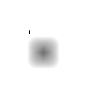
\begin{tikzpicture}
    % draw the shadow
    \foreach \x in {0,0.05,...,1} {
      \setlength{\shadowiter}{\boxshadowsize*\real{\x}}
      \fill[xshift=\boxshadowsize-1pt,yshift=-\boxshadowsize+1pt,
          black,opacity=0.04,rounded corners=\boxroundness]
          (\shadowiter,\shadowiter) rectangle +(\boxw-2\shadowiter,\boxh-2\shadowiter);
    }
    % draw the box border
    \filldraw[fill=\fillcolor,draw=\drawcolor,rounded corners=\boxroundness]
        (0,0) rectangle (\boxw,\boxh);
    % draw the content
    \node[xshift=\boxroundness,yshift=\boxroundness,inner sep=\innersep,outer sep=0pt,anchor=south west]
        at (0,0) {\usebox{\shadowblockbox}};
  \end{tikzpicture}
}

\newcommand\gitcmd[1]{%
%\begin{center}
%  \noindent\fcolorbox{white}{yellow!20}{%
%    \begin{minipage}{.7\textwidth}
%      \centering\Large
%      \texttt{#1}
%    \end{minipage}}
%\end{center}

\begin{center}
  \begin{shadowblock}{0.9\textwidth}{yellow!50}{black!50}{0pt}
  \centering\Large
  \texttt{#1}
  \end{shadowblock}
\end{center}
}

%\newsavebox{\framedtextbox}
%\newenvironment{framedtext}[1] % minipage width
%{\begin{lrbox}{\framedtextbox}\begin{minipage}{#1}\centering}
%{\end{minipage}\end{lrbox}
%  % put box in a tikz node, and draw the node.
%  \begin{tikzpicture}
%    \node [fill=gray!20,rounded corners] at (0,0) {\usebox{\framedtextbox}};
%  \end{tikzpicture}
%}
\newenvironment{framedtext}
{\begin{center}\begin{shadowblock}{0.7\textwidth}{gray!20}{red}{10pt}\ttfamily}
{\end{shadowblock}\end{center}}

\newcommand\surrounded[1]{
  \textless#1\textgreater
}

\newcommand\optionalSurrounded[1]{
  [\textless#1\textgreater]
}


\sybtitle{Android中的智能指针}
\sybauthor{孙延宾}
\sybdate{\today}

\begin{document}
\tt % I love Typewriter font.
%%%%%%%% the title page and toc %%%%%%%%%%
\pagestyle{header}
\sybmaketitle
\tableofcontents
\newpage

%%%%%%% the main content %%%%%%%%%
\pagestyle{main}
\setcounter{page}{1}

\section[一般的智能指针]{一般的智能指针}
智能指针的概念在C++的世界中比较常见,它的出现是为了解决两个经典问题:
\begin{itemize}
\item object生命周期结束后如何自动释放其占有的内存?
\item 如何避免出现野指针?
\end{itemize}
第一个问题处理不好就会出现内存泄露,而第二个问题就是空指针,两个都是非常严重的
问题。

智能指针的概念就是为了解决这两个问题而提出的,它的思路是为对象创建一个管理器,
这个管理器也是一个对象(叫做影子对象),通过指针关联到我们真正在意的对象(就叫做
本体吧),我们不直接操作本体而是操作影子对象,这是通过在影子对象中重载“.”和
“->”两个操作实现的,也就是我们调用影子对象的方法时,实际调用的是本体中的方法,
由此可见,我们是无法通过影子对象访问本体中的属性的。
影子对象中保有一个计数器,记录它被引用的次数(注意是影子
对象被引用的次数,因为我们操作影子对象,即使我们的本意是引用本体),每次增加
引用时计数加一,引用完毕之后计数减一,等到计数为零时,影子对象将本体和自己
一并释放,引用者无需额外操作。

那么,智能指针具体是如何解决上述两大问题的呢?

1. 影子对象是于stack上的,所以其生命周期结束后会自动释放(见CPP notes的相关章节),
我们只需在其析构函数中减少影子对象的计数器即可,等计数器减到零时,影子对象自会
释放本体和它自身所占用的内存,第一个问题完美解决了。

2. 由于我们只跟影子对象打交道,所以只要影子对象中的计数不出错,本体是不会被意外
销毁的,也就不会出现野指针了,第二个问题完美解决了。

\section[Android中的智能指针]{Android中的智能指针}
使用智能指针是否就万事大吉了呢,很可惜,不能!现实世界中还有一类programmer经常
会犯的错误:循环引用,而智能指针无法解决此类问题,Android中为此修改了智能指针
的实现,变为强弱指针,不过这仍然不能完全解决循环引用的问题:强指针与强指针相互
引用时Android也无能为力了,这是需要programmer需要关注的。

\section[数据结构]{数据结构}
基类,所有使用智能指针的类必须继承该基类。

\begin{cppcode}
// base class of interface: RefBase
class RefBase {
// data
private:
    weakref_impl* const mRefs;

// method
public:
    // strong pointer operations
    void incStrong();
    void decStrong();
    void forceIncStrong();

    // operations for weak pointer
    weakref_type* createWeak();
    weakref_type* getWeakRefs();

    // change lifetime controller, strong or weak
    void extendObjectLifetime(int32_t mode);

    // interface for subclass
    void onFirstRef();
    void onLastStrongRef();
    void onLastWeakRef();
    void onIncStrongAttempted(uint32_t flags, void* id);
}
\end{cppcode}

每个基类对象都有一个计数器对象,负责记录引用计数。

\begin{cppcode}
// 计数器对象: weakref_imple
class RefBase::weakref_impl : public RefBase::weakref_type {
// data
public:
    int32_t mStrong; // 强引用计数
    int32_t mWeak;   // 弱引用计数
    RefBase* mBase;  // 本体对象
    int32_t mFlags;  // 生命周期标志

// methods
    RefBase* refBase();  // 获取本体对象
    void incWeak();
    void decWeak();
    bool attemptIncStrong();
    bool attemptIncWeak();
}
\end{cppcode}

强指针类,只有一个本体对象的指针,在构造函数中增加引用计数,
在析构函数中减少引用计数。

\begin{cppcode}
// strong pointer class: sp
template <typename T>
class sp {
// data
private:
    T* m_ptr;  // 本体对象指针

// methods
public:
    sp();
    ~sp();
    T* get() { return m_ptr; }
    void clear();  // 修改引用计数
}
\end{cppcode}

弱指针类,构造函数、析构函数中只增、减弱引用计数,
弱指针不能直接调用本体对象,必须提升为强指针才行。

\begin{cppcode}
// weak pointer class: wp
template <typename T>
class wp {
// data
private:
    T* m_ptr;  // 本体对象的指针
    weakref_type* m_refs;  // 本体计数器对象的指针

// methods
public:
    wp();
    ~wp();
    weakref_type* get_refs() { return m_refs; }
    T* unsage_get() { return m_ptr; }
    sp<T> promote();  // 弱指针只能提升为强指针才能使用
    void clear();  // 修改引用计数
}
\end{cppcode}

\section[强指针对象]{强指针对象}
操作思路:

创建强指针对象时,创建本体对象,并在class sp的构造函数中增加强、弱引用计数,
初次创建本体对象时,调用子类接口onFirstRef()。

通过强指针对象调用本体对象的方法:强指针对象重载“.”和“->”操作符了。

强指针对象销毁时,减少本体对象的强、弱引用计数,如果强引用计数减为0时,

\begin{cppcode}
call subclass interface: onLastStrongRef();
if(lifetime controlled by strong ref) {
  delete 本体对象;
}
\end{cppcode}

弱引用计数减少到0时,

\begin{cppcode}
if(lifetime controlled by strong ref) {
  // 此时本体对象已经被销毁了,因为强引用计数<=弱引用计数
  delete ourself;
} else {
  // 证明周期有弱引用计数控制,所以强引用计数减为0时并没有销毁本体对象,
  // 我们在此销毁它
  call subclass interface: onLastWeakRef();
  delete mBase;
}
\end{cppcode}

\section[弱指针对象]{弱指针对象}
弱指针对象跟强指针对象类似,主要区别有二:
1. 弱指针对象创建、销毁只影响本体对象的弱引用计数,不涉及强引用计数。

2. 无法通过弱指针对象操作本体对象,因为弱指针对象没有重载“.”和“->”操作符,
只有通过弱指针对象的promote()方法拿到强指针之后才能操作本体对象,注意如果
m\_ptr==NULL,说明本体对象一定不,那么promte()一定失败,所以就不用再尝试了;
m\_ptr!=NULL不能确保本体对象一定就存在,还需要进行判断,判断通过attemptIncStrong()
函数进行。

下面看attemptIncStrong()函数:

\begin{cppcode}
// 正常情况
if(0 < 强引用计数 < 初始值) {
  增加强、弱引用计数;
  return true; // 升级成功!
}

bool allow = false;

if(强引用计数 == 初始值) {
  // 这说明本体对象创建之后还从未被强引用过,而此时又有弱引用,考虑:
  // wp<Interface> w = new Interface();
  // 这样的情形,此时本体对象需要弱引用计数为0时才会释放,而当前弱引用
  // 不为0
  if(lifetime controlled by strong ref)
    allow = true;
}

if(强引用计数 <= 0) {
  // 本体对象被强引用过啊,如果生命周期由强引用计数控制就死定了
  if(lifetime controlled by weak ref)
    allow = true;
}

if(allow)
  incStrong();
if(原始强引用计数 == 初始值) {
  android_atomic_add(-INITIAL_STRONG_VALUE, &impl->mStrong);
  call subclass interface: onFirstRef();
}

return true;
\end{cppcode}

\section[强弱指针如何防止循环引用]{强弱指针如何防止循环引用}
假设A、B循环引用,C是A-B系统外的引用,C引用A。A,B生命周期均为strong的。

1. A, B相互强引用,C强引用A。

C断开对A的引用时,此时Android无能为力,A,B均无法释放。

2. A强引用B,B弱引用A,C强引用A。

C断开对A的强引用时,A的strong ref为0,销毁之;这时A断开对B的强引用,
B的strong ref又变成0了,销毁之,于是循环引用被破解。

3. A弱引用B,B强引用A,C强引用A。

这种情况不存在,因为此时B不存在强引用,早就销毁了。

\section[总结]{总结}
使用中应注意,在可能存在循环引用的地方使用强、弱引用以防止循环引用,此时就
应该设置从属关系,哪个主哪个仆就要看个人设计了,如binder中,client强引用
service的对象,service则通过弱引用链接client中的death recipient,service为主,
client为仆。

\end{document}